\section{Methodology}

\subsection{Research questions}

We structure our research through the following research questions:

\begin{itemize}
    \item[\textbf{RQ1}] Are ownership metrics indicative for the presence of implicated code in source files for open-source software projects?
    
    \item[\textbf{RQ2}] Can ownership metrics be used to build a classification model to identify implicated source files?
    \begin{itemize}
        \item[\textbf{2a}] For which level of granularity (line-based or commit-based) do ownership metrics give more accurate results when used to build the classification model?
        \item[\textbf{2b}] How does the value of the threshold, used to distinguish minor and major contributors, impacts on the accuracy of the classification model?
    \end{itemize}
    % \item[\textbf{2a}] For which level of granularity (line-based or commit-based) do ownership metrics give more accurate results when used to build the classification model?
    
    % \item[\textbf{2b}] How does the value of the threshold, used to distinguish minor and major contributors, impacts on the accuracy of the classification model?
\end{itemize}

The first research question is a more general question, which is needed to determine if in general ownership metrics can be a good indication of the presence of implicated code in source files for open-source software. 
The second research question focuses on if it is possible to classify the implicated files based on ownership metrics. The sub-questions focus on the type of metrics included in the classifier: in particular on the parameters used to compute them (i.e. code changes granularity and minor-major threshold) and on the effects resulting from changing these parameters. %: which granularity (line or based) gives the best results, and if the minor-major threshold plays a significant role in classifying.

%In previous research, ownership has always been related to the amount of commits done by a specific contributor, but are there other ways to compute ownership that give a better result in terms of relationship with implicated files? The last research question focuses on the threshold to determine major or minor contributors. In previous research arbitrary values had been chosen for the threshold, but does have di

\subsection{Study subjects}
\label{sec:subjects}
A software project, in order to be used for this research, should (1) be and open-source software project; (2) use git as version control system, or have a git mirror of the repository (requirement for the technique described in Section~\ref{sec:implicated}; (3) use JIRA as issue tracking system and adhere to the Apache JIRA convention, so that we can apply the technique described in Section~\ref{sec:bug-linking}.

We selected five different software projects as study subjects, all written using the Java programming language. In Table~\ref{tab:projects} we show some information about each one of them. When choosing the projects we checked if they satisfied the previous mentioned requirements, but also tried to choose them with different sizes and application fields, in order to have a diverse group.

For each project we decided to  consider its whole development history until the 01/01/2015: this because we had issues extracted in JSON until the half of the year, and we only wanted to consider code for which the most of the issues were already discovered and fixed. We also decided to discard some of the first days of commits from the data extracted from the repositories, because these are the commits needed to setup the project repository or the git mirror. %As a result they commit sometimes years of data in one commit so the whole history there is lost. 
We did this last step by manually checking the messages of the first available commits.

\begin{table*}[ht]
\centering
\caption{Characteristics of the studied projects %over their history
(until 01/01/2015)}
\label{tab:projects}
\footnotesize
\begin{tabular}{|l|c|c|c|c|c|}
\hline
\textbf{Project} & \textbf{LOC} & \textbf{Contributors} & \textbf{Commits} & \textbf{Application} \\%& \textbf{Period}\\
\hline
Camel   & 103883  & 125 & 18371  & Rule-based routing and mediation engine \\
\hline
Lucene-solr & 220632 & 55 & 13841  & Information retrieval library and search platform\\
\hline
Mahout      & 177317 & 31 & 3163 &   Implementation of scalable machine-learning algorithms \\
\hline
Maven       & 129132 & 51 & 9909 &   Build manager \\
\hline
Zookeeper   & 108132 & 13  & 1283 &  Distributed system configuration service \\
\hline
\end{tabular}
\end{table*}


\subsection{Research steps}

What we want to do is to build a model that is able to identify the implicated files in the history of the selected software projects, and to evaluate its effectiveness. In this Section we describe in a detailed way all the steps followed in this research.

\subsubsection{Project history dataset}
\label{sec:history-dataset}

In the first step of our research we create, for every software project, a dataset that contains all its Java files history (over the considered time period, see Section~\ref{sec:subjects}) in terms of commits, lines, bug fixes and implications. To do that we go through all the commits in its \textit{git log}, and for every commit we:
\begin{enumerate}
\item extract the list of the Java files affected; 
\item for each affected file update the information about the contribution that the author of the commit performed to it in terms of lines added, lines deleted and number of commits;
\item extract information about the file itself: size (LOC), authorship information, comment lines, if it is a bug fix (using the technique described in Section~\ref{sec:bug-linking});
\item add to the data set, for each one of these files, as many lines as the number of authors that contributed to it until the considered commit (included): each one of these lines contains the information about the contribution of the corresponding author to the corresponding file, at the moment of the corresponding commit, plus the information related to the commit itself.
\end{enumerate}

We then add to this dataset, once extracted, another column that says when a file is implicated, using the approach described in Section~\ref{sec:implicated}.

A complete list of the columns contained in the dataset can be found in
\Cref{tab:modeled_information}. Some of them contain information that are not related to the single author, but to the file or the commit: in this case their value will be the same for more than one line.

An example of this procedure is shown in Figure~\ref{fig:history_example} and Table~\ref{tab:history_example}, it shows only information about commits and lines added but it can be used to better understand the described methodology.

\begin{figure}[ht]
    \centering
    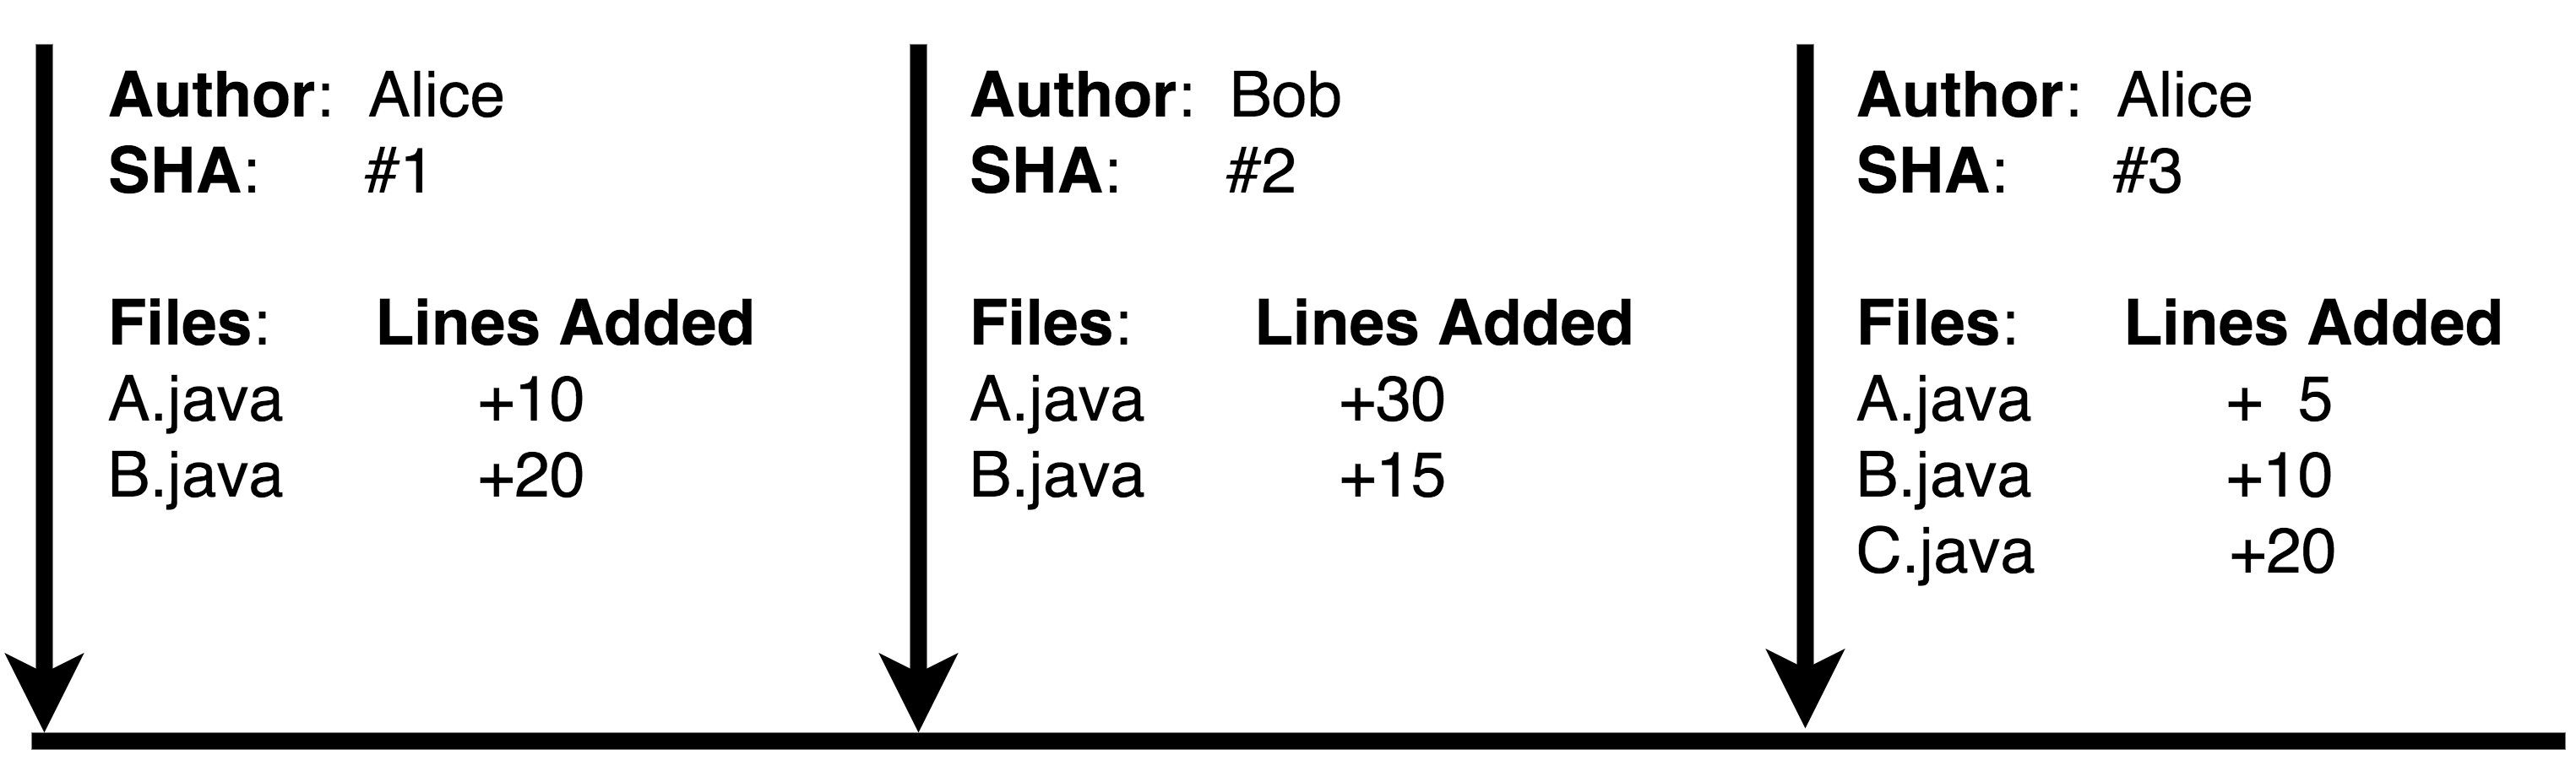
\includegraphics[width=0.48\textwidth]{images/history_example.png}
    \caption{Example of a small portion of development history (i.e. commits), with lines added information. The corresponding history dataset is shown in Table~\ref{tab:history_example}}
    \label{fig:history_example}
\end{figure}

\begin{table}[ht]
\centering
\footnotesize
\begin{tabular}{|c|c|c|c|c|c|c|c|}
\cline{3-8}
\multicolumn{1}{c}{} & 
\multicolumn{1}{c}{} & \multicolumn{6}{|c|}{\textbf{columns (see \Cref{tab:modeled_information})}} \\
\hline
\textbf{file} & \textbf{sha} & \textbf{4} & \textbf{5} & \textbf{6} & \textbf{7} & \textbf{11} & \textbf{12}
\\
\hline
A.java & \#1 & Alice  & 10                        & 10                                & 10               & 1                     & 1                  \\
B.java & \#1 & Alice  & 20                        & 20                                & 20               & 1                     & 1                  \\
A.java & \#2 & Alice  & 10                        & 0                                 & 40               & 1                     & 2                  \\
A.java & \#2 & Bob    & 30                        & 30                                & 40               & 1                     & 2                  \\
B.java & \#2 & Alice  & 20                        & 0                                 & 35               & 1                     & 2                  \\
B.java & \#2 & Bob    & 15                        & 15                                & 35               & 1                     & 2                  \\
A.java & \#3 & Alice  & 15                        & 5                                 & 45               & 2                     & 3                  \\
A.java & \#3 & Bob    & 30                        & 0                                 & 45               & 1                     & 3                  \\
B.java & \#3 & Alice  & 30                        & 10                                & 45               & 2                     & 3                  \\
B.java & \#3 & Bob    & 15                        & 0                                 & 45               & 1                     & 3                  \\
C.java & \#3 & Alice  & 20                        & 20                                & 20               & 1                     & 1 \\\hline
\end{tabular}
\caption{Example of a small portion of history dataset with a reduced set of columns. The corresponding development history is shown in Figure~\ref{fig:history_example}}.
\label{tab:history_example}
\end{table}

\begin{table}[ht]
\centering
\footnotesize
\begin{tabular}{|c|c|c|c|c|c|c|c|c|}
\cline{3-9}
\multicolumn{1}{c}{} & 
\multicolumn{1}{c}{} & \multicolumn{7}{|c|}{\textbf{columns (see Table~\ref{tab:metrics})}} \\
\hline
\textbf{sha} & \textbf{file} & \textbf{3} & \textbf{4} & \textbf{6} & \textbf{11} & \textbf{12} & \textbf{13} & \textbf{14}
\\
\hline
\#1 & A.java & 1 / 1             & 10 / 10                & 1                   & 1                   & 0                   & 1                                 & 0                                 \\
\#1 & B.java & 1 / 1             & 20 / 20                & 1                   & 1                   & 0                   & 1                                 & 0                                 \\
\#2 & A.java & 1 / 2             & 30 / 40                & 2                   & 2                   & 0                   & 1                                 & 1                                 \\
\#2 & B.java & 1 / 2             & 20 / 35                & 2                   & 2                   & 0                   & 2                                 & 0                                 \\
\#3 & A.java & 2 / 3             & 30 / 45                & 2                   & 2                   & 0                   & 2                                 & 0                                 \\
\#3 & B.java & 2 / 3             & 30 / 45                & 2                   & 2                   & 0                   & 2                                 & 0                                 \\
\#3 & C.java & 1 / 1             & 20 / 20                & 1                   & 1                   & 0                   & 1                                 & 0                 
\\ \hline
\end{tabular}
\caption{Example of a small portion of metrics dataset with a reduced set of columns, extracted from the history dataset example shown in Table~\ref{tab:history_example} using a 30\% threshold to distinguish minor and major contributors.}
\label{tab:metrics_example}
\end{table}

\begin{table*}[ht]
\centering
\caption{Information modeled and stored in our dataset, per committed file}
\label{tab:modeled_information}
\begin{tabular}{|l|l|p{0.65\textwidth}|}
\hline
\# & \textbf{Column} & \textbf{Description}  \\\hline
\hline
1 & project & 
    project name \\ \hline
2 & file & 
    file name (full path)\\ \hline
3 & sha & 
    commit SHA (also, file revision) \\ \hline
4 & author & 
    contributor's name \textbf{(NOTE: it is not the author of the commit, but one of the file contributors)} \\ \hline
5 & author\_file\_tot\_added & 
    total lines added by the author to the file\\ \hline
6 & author\_file\_added\_this\_commit & 
    lines added by the author to the file with the commit (different from 0 only for the author of the commit)\\ \hline
7 & file\_tot\_added & 
    total lines added to the file\\ \hline
8 & author\_file\_tot\_deleted & 
    total lines deleted by the author from the file\\ \hline
9 & author\_file\_deleted\_this\_commit & 
    lines deleted by the author from the file with the commit (different from 0 only for the author of the commit)\\ \hline
10 & file\_tot\_deleted & 
    total lines deleted from the file\\ \hline
11 & author\_file\_commits & 
    total commits to the file by the author\\ \hline
12 & file\_tot\_commits & 
    total commits to the file\\ \hline
13 & current\_lines\_authored & 
    number of lines actually present in the file and authored by the author (obtained from the \textit{git blame} output)\\\hline
14 & current\_file\_size & 
    file size measured in LOC (lines of code)\\\hline
15 & current\_comment\_lines & 
    comments size in terms of lines\\\hline
16 & max\_current\_author & 
    number of lines actually present in the file and authored by the author that authored the highest number of lines actually in the file (obtained from the \textit{git blame} output)\\\hline
17 & total\_current\_authors & 
    number of authors of the lines actually present in the file (obtained from the \textit{git blame} output)\\\hline
18 & commit\_date & date of the commit\\ \hline
19 & bug\_fix & 1 if the commit fixes one or more bugs, zero otherwise\\ \hline
20 & fixed\_bugs & JIRA KEY-ID of the bugs fixed, empty if the commit is not a bug fix\\ \hline
21 & affected\_versions & list of the project releases affected by the bugs fixed by the commit, empty if the commit is not a bug fix\\ \hline
22 & implicated & 1 if the file version is implicated \\ \hline
\end{tabular}
\end{table*}


\subsubsection{Metrics computation}
\label{sec:metrics}
In this second step, for every project and using the respective history
dataset, we compute the dataset that contain the metrics that we need for the
classification. We need to compute the metrics for every version of every file,
so the computation is done grouping by commit SHA and file (columns 2 and 3 of
the history dataset, see \Cref{tab:modeled_information}). 

As metrics we compute the ownership ones described in
Section~\ref{sec:ownership-metrics} together with the classic code metrics
listed in Section~\ref{sec:classification-overview}. This will produce another
data set, with fewer lines, that contains the metrics and the column
``implicated'', defined as in \Cref{tab:modeled_information}. A complete set of the columns of the metrics dataset can be seen in Table~\ref{tab:metrics}, where the terms ownership, minor, major and total must be interpreted as defined in Section~\ref{sec:ownership-metrics}. 

A different version of this dataset is computed for every threshold listed in Section~\ref{sec:ownership-metrics} (the threshold used to distinguish minor and major contributors).
Table~\ref{tab:metrics_example} shows an example of the metrics dataset resulting from the history dataset example shown in Table~\ref{tab:history_example}, using a threshold of 30\%; it contains a reduced set of columns: only the ones based on the lines added and on the commit count.

\begin{table*}[t]
\centering
\caption{Columns of the metrics dataset;  See
Section~\ref{sec:ownership-metrics} and \Cref{tab:modeled_information} for the terms used in the definitions.}
\label{tab:metrics}
\footnotesize
\begin{tabular}{|l|l|p{0.65\textwidth}|}
\hline
\# & \textbf{Column} & \textbf{Description}  \\
\hline
1 & sha & 
    commit SHA (can be interpreted as file version or revision) \\ \hline
2 & file & 
    file name (full path)\\ \hline
3 & commit\_ownership & 
    max( author\_file\_commits / file\_tot\_commits)\\ \hline
4 & line\_ownership\_added & 
    max( author\_file\_tot\_added / file\_tot\_added)\\ \hline
5 & line\_ownership\_deleted & 
    max( author\_file\_tot\_deleted / file\_tot\_deleted)\\ \hline
6 & total\_contributors & 
    total number of contributors (count the of the lines grouped together) \\ \hline %since for a specific file and sha there are as many lines as the number of contributors in the history dataset)
7 & line\_authorship & 
    max\_current\_author / file\_size \\ \hline
8 & total\_authors & 
    total\_current\_authors\\ \hline
9 & file\_size & 
    file\_size\\ \hline
10 & comment\_to\_code\_ratio & 
    current\_comment\_lines / (current\_file\_size - current\_comment\_lines)\\ \hline
11 & major\_contributors & 
    count where author\_file\_commits / file\_tot\_commits >= threshold\\ \hline
12 & minor\_contributors & 
    count where author\_file\_commits / file\_tot\_commits < threshold\\ \hline
13 & lines\_added\_major\_contributors & 
    count where author\_file\_tot\_added / file\_tot\_added >= threshold\\ \hline
14 & lines\_added\_minor\_contributors & 
    count where author\_file\_tot\_added / file\_tot\_added < threshold\\ \hline
15 & lines\_deleted\_major\_contributors & 
    count where author\_file\_tot\_deleted / file\_tot\_deleted >= threshold\\ \hline
16 & lines\_deleted\_minor\_contributors & 
    count where author\_file\_tot\_deleted / file\_tot\_deleted < threshold\\ \hline
17 & previous\_implications &
    count how many times this file was implicated before that version\\\hline
18 & implicated & 1 if the file version is implicated \\\hline
\end{tabular}
\end{table*}

\subsubsection{Classification}
Using the metrics dataset we build, for every project, a classification model using the Random Forests approach~\cite{breiman2001random}, and we then evaluate how effective it is when used to distinguish which file versions are implicated. We also use Logistic Regression to determine which features are significant. The choice of these techniques is based on the fact that they were already used respectively in~\cite{Greiler:replication} and~\cite{bird:original}. An accurate description of this process is provided in Section~\ref{sec:evaluation}.


% Correlation and classification of buggy files/commits.
%\subsubsection{Statistical approach}
%The features will be used to see if there is a correlation between them and the fact that a file is implicated. For the classification we will use the \textit{Random Forest} classification algorithm.



% Compute metrics for all commits and all files changed by that commit

% Find all implicated code by finding all fixing commits and using git diff and blame to find the commits when those lines where last modified.


% New data set (for the Lucene projects) that contains:
% - All the history of the commits
% For every commit, all the files changed
% For every file changed, author ownership (at the time of the commit) and bug information (implicated, fix, etc.)
% Ownership metrics computation (different granularities) and Exploratoty Data Analysis → determine minor / major threshold
% Correlations and classification of buggy files/commits
% Replicate on more OSS projects



% The dataset of every project contains several field, which contain data specific to the commit, file, and author. The dataset contain the following fields:



% From this dataset different kinds of ownership metrics will be extracted, which will be used to find a correlation with code quality.[h
